\medskip

\textbf{Partie A : étude de la fonction }\boldmath$f$\unboldmath

\medskip

La fonction $f$ est définie sur l'intervalle $]0 ~;~+\infty[$ par : 

\[f(x)=x-2+\dfrac{1}{2} \ln x,\]
 où ln désigne la fonction logarithme népérien. On admet que la fonction $f$ est deux fois dérivable sur $] 0 ~;~ +\infty[$, on note $f'$ sa dérivée et $f''$ sa dérivée seconde.

\begin{enumerate}
	\item \begin{enumerate}
		\item Déterminer, en justifiant, les limites de $f$ en 0 et en $+\infty$.

		\item Montrer que pour tout $x$ appartenant à $] 0 ~;~+\infty[$, on a :\quad $f'(x)=\dfrac{2x + 1}{2x}$.

		\item Étudier le sens de variation de $f$ sur $] 0 ~;~+\infty[$.

		\item Étudier la convexité de $f$ sur $] 0~;~ +\infty[$.
	\end{enumerate}

	\item \begin{enumerate}
		\item Montrer que l'équation $f(x)=0$ admet dans $] 0 ~;~ +\infty[$ une solution unique qu'on notera $\alpha$ et justifier que $\alpha$ appartient à l'intervalle $[1~;~2]$.

		\item Déterminer le signe de $f(x)$ pour $x \in] 0 ~;~ +\infty[$.

		\item Montrer que $\ln (\alpha)=2(2-\alpha)$.
	\end{enumerate}
\end{enumerate}

\medskip

\textbf{Partie B : étude de la fonction }\boldmath $g$\unboldmath

\smallskip

La fonction $g$ est définie sur $] 0~;~1]$ par :

\[g(x) = -\dfrac{7}{8} x^{2}+ x - \dfrac{1}{4} x^{2} \ln x.\]

On admet que la fonction $g$ est dérivable sur $] 0~;~1]$ et on note $g'$ sa fonction dérivée.

\begin{enumerate}
	\item Calculer $g'(x)$ pour $x \in ] 0~;~1]$ puis vérifier que $g'(x)=x f\left(\dfrac{1}{x}\right)$.

	\item \begin{enumerate}
		\item Justifier que pour $x$ appartenant à l'intervalle $\left] 0~;~\dfrac{1}{\alpha}\right[$, on a $f\left(\dfrac{1}{x}\right)>0$.

		\item On admet le tableau de signes suivant :

		\begin{center}
			\begin{tikzpicture}
				\tkzTabInit[lgt=3]{$x$/1,signe de $f\left(\dfrac{1}{x}\right)$/1.3 }{0,$ \dfrac{1}{\alpha } $,1}
				\tkzTabLine{d,+,z,-,}
			\end{tikzpicture}
		\end{center}

		En déduire le tableau de variations de $g$ sur l'intervalle $] 0~;~1]$. Les images et les limites ne sont pas demandées.
		\end{enumerate}
	\end{enumerate}

\medskip

\textbf{Partie C : un calcul d'aire.}

\smallskip

On a représenté sur le graphique ci-dessous :

\begin{itemize}
\item La courbe $\mathcal{C}_{g}$ de la fonction $g$;

\item La parabole $\mathcal{P}$ d'équation $y=-\dfrac{7}{8} x^{2}+x$ sur l'intervalle $]0~;~1]$.

\end{itemize}

\begin{center}
				\begin{tikzpicture}[x =100mm,y = 100mm]
					\draw [color = gray!75, line width = 1pt, xstep=0.1,dashed, ystep = 0.1] (0,0) grid (1.05,0.45);
					\draw[->] (0.03,0) -- (1.05,0);
					\foreach \x/\l in {0.1/{$ \np{0.1} $},1/{1},0.579/{$ \dfrac{1}{\alpha} $}}
					\draw[shift={(\x,0)},color=black] (0pt,2pt) -- (0pt,-2pt) node[below, fill = white] {\footnotesize \l};
					\draw[->] (0,-0.03) -- (0,0.45);
					\foreach \y in {0.1}
					\draw[shift={(0,\y)},color=black] (2pt,0pt) -- (-2pt,0pt) node[left, fill = white] {\footnotesize $\np{\y}$};
					\draw[color=black] (-2pt,-2pt) node[below left] {{\footnotesize O}};
					\draw[samples=100,domain= 0.579:1,pattern = north east lines ,fill opacity=0.4] plot(\x, {-7*\x*\x/8+\x-0.25*\x*\x*ln(\x)})--plot({(1.579-\x)}, {-7*(1.579-\x)*(1.579-\x)/8+1.579-\x});
					\draw[line width=1.2pt,color=red,smooth,samples=100,domain= 0.0001:1] plot(\x, {-7*\x*\x/8+\x-0.25*\x*\x*ln(\x)});
					\draw[line width=1.2pt,color=red,smooth,samples=100,domain= 0.0001:1] plot(\x, {-7*\x*\x/8+\x});
					\draw[dashed,line width=1.5pt] (0.579,0)--(0.579,0.331) (1,0)--(1,0.125);
					\node at (0.75,0.33){$ \mathcal{C}_g $};
					\node at (0.75,0.23){$ \mathcal{P} $};
				\end{tikzpicture}
			\end{center}


On souhaite calculer l'aire $\mathcal{A}$ du domaine hachuré compris entre les courbes $\mathcal{C}_{g}$ et $\mathcal{P}$, et les droites d'équations $x=\dfrac{1}{\alpha}$ et $x=1$.

On rappelle que $\ln (\alpha)=2(2-\alpha)$.

\begin{enumerate}
	\item \begin{enumerate}
		\item Justifier la position relative des courbes $C_{g}$ et $\mathcal{P}$ sur l'intervalle $\left.] 0~;~1\right]$.

		\item Démontrer l'égalité :

			$$
			\int_{\frac{1}{\alpha}}^{1} x^{2} \ln x \:\mathrm{d}x=\dfrac{-\alpha^{3}-6 \alpha+13}{9 \alpha^{3}}
			$$

	\end{enumerate}

	\item En déduire l'expression en fonction de $\alpha$ de l'aire $\mathcal{A}$.
\end{enumerate}
